\chapter{مقدمه}

\section{مقدمه}

در این فصل ابتدا به بیان هدف پروژه و انگیزه از طرح آن پرداخته می‌شود. سپس دلیل نیاز و فواید سیستم‌های چندعاملی پرداخته خواهد شد. در ادامه به تاثیر هوش مصنوعی در رباتیک اشاره خواهد شد و در انتها شمای کلی از فصل‌های پایان‌نامه ارائه می‌شوند.

\section{هدف و انگیزه}
امروزه با توسعه هوشمندسازی، انواع مختلف ربات‌ها با توانمندی‌های متنوع مورد استفاده قرار می‌گیرند. عملکرد گروه ربات‌ها و تعامل بین آن‌ها در صنایع مختلف کاربرد دارد. که یکی از انواع آن، سیستم چند عاملی\LTRfootnote{multi-agent systems} و به طور خاص اجماع\LTRfootnote{platoon} است. منظور از اجماع دسته‌ای از ربات‌هاست که به هدایت یکی از آن‌ها، در کنار یکدیگر با نظم و ترتیب، فاصله استاندارد و با سرعت بهینه در کنار یکدیگر حرکت کنند.

در این پروژه هدف کنترل ربات‌های چرخ‌دار متحرک\LTRfootnote{mobile wheeled robots}، مدل دیفرانسیلی\LTRfootnote{differential model}، نیمه خودران و پیاده‌سازی اجماع ربات‌ها است که این سیستم به کمک شبیه‌ساز\LTRfootnote{Simulink} متلب\LTRfootnote{MATLAB} و برای نمایش به کمک ابزار شبیه سازی ربات‌های متحرک\LTRfootnote{mobile robotics simulation toolbox} پیاده سازی گردیده است.

با بهره‌گیری از فناوری اینترنت اشیاء\LTRfootnote{Internet of Things} می‌توان ارتباط ربات‌ها را در بستر اینترنت به یکدیگر و یا به مراکز مختلف میسر نمود. به این ترتیب می‌توان به کمک آن برای ربات‌ها مسیر طراحی‌ و ترافیک مسیر و اجماع ربات‌ها را تا رسیدن به مقصد کنترل کرد.

از مزایای اجماع عبارت از تسریع در عملیات‌ و کاهش انرژی مصرفی و استهلاک ربات‌ها است. از جمله کاربردهای دسته‌ای می‌توان به خودروهای سنگین نیمه هوشمند بین شهری، در جاده‌های اختصاصی شرکت‌ها برای جابه‌جایی مواد اولیه و فراورده‌ها و درون انبارها اشاره کرد. همچنین در جابه‌جایی اجسامی که یک ربات به تنهایی از انجام آن ناتوان است، در عملیات‌های امدادی جست و جو و حتی در فضا دسته‌ای استفاده می‌گردد که نشان از اهمیت بسیار بالای آن است.

امروزه علم مدیریت ترافیک با ترکیب تکنولوژی‌های پیشرفته با زیر ساخت‌های شهری، بسیار نوین گشته است. این امر باعث جذب علاقه مدیران برای استفاده از سازمان حمل و نقل هوشمند\LTRfootnote{Intelligent Transportation System} شده است \cite{baskar2011traffic}. رکن اصلی سازمان حمل و نقل هوشمند خودرو هوشمند\LTRfootnote{intelligent vehicle} است. خودروهای هوشمند دارای ویژگی‌هایی هستند که از مهمترین آن‌ها می‌توان به خودران\LTRfootnote{autonomous vehicles} بودن خودروها اشاره کرد.

خودران بودن خودروها علاوه بر اینکه راحتی و وقت بیشتر به خاطر آزاد بودن سرنشینان را به همراه دارد، می‌تواند از اشتباه‌های رانندگان خودروها نیز جلوگیری و به راحتی مدیریت کرد. در نتیجه ترافیک کمتر و امنیت بیشتری را در سطح جاده‌ها فراهم آورد.

ایده جذاب دیگر این است که به جای کنترل یک خودرو، گروهی از خودروها را کنترل کرد. به این ترتیب که هر خودرو وظیفه مسیریابی نداشته باشد و بتوان الگوریتم‌های مسیریابی را بهینه کرد. برای مثال می‌توان فاصله خودروها را به نسبت سرعتشان کمتر کرد تا از ظرفیت جاده‌ها بیشتر استفاده گردد.

موضوع مهم دیگر رابطه هوش مصنوعی\LTRfootnote{artificial intelligence} و رباتیک است. رباتیک بر پایه پیشرفت‌های ایجاد شده در مکاترونیک، مهندسی برق و محاسبه، عملکرد موتورهای سنسورداری را که قابلیت وفق دادن خود با محیط همیشه در حال تغییر را دارند، ارتقا می‌دهد. تا به حال، سیستم‌های صنعتی، به صورت محیط مناسب برای توانایی‌ها و ویژگی‌های ربات ساخته می‌شد اما امروزه ربات‌ها می‌توانند در محیط‌‌های مختلفی خود را وفق دهند.
اتوماسیون ربات، می‌تواند به سه دسته ادراک\LTRfootnote{perceiving} ، برنامه‌ریزی\LTRfootnote{planning} و اجرا\LTRfootnote{execution} (اثرگزاری\LTRfootnote{manipulating}، پیمایش\LTRfootnote{navigating} و همکاری\LTRfootnote{collaborating}) تقسیم شود. هدف از ادغام هوش مصنوعی و رباتیک، بهینه‌کردن اتوماسیون\LTRfootnote{automation} با یادگیری است. این سطح از هوش را می‌توان با توانایی پیشبینی آینده، چه در برنامه‌ریزی یک عمل یا تعامل با محیط، اندازه‌گیری کرد. با وجود اینکه ساخت سیستمی که همانند انسان هوشمند باشد، هنوز موفقیت‌آمیز نبوده است، ربات‌ها امروزه قادر به انجام کارهای بسیار تخصصی‌ای مثل راندن خودرو، پرواز در محیط‌های طبیعی و ساخته انسان، شنا، حمل جعبه و اجسام در ناحیه‌های مختلف، برداشت و قرار دادن اجسام، هستند \cite{perez2018artificial}.

در این پایان‌نامه الگوریتم‌های هوش مصنوعی برای مسیریابی دسته‌ی ربات‌ها مورد بررسی و مقایسه قرار گرفته‌اند تا بهترین روش در این بین برای مسیریابی ربات‌ها، از نظر زمانی، مسافت و امنیت یافت شود.

\section{کارهای پیشین}
دانشمندان و محققان زیادی برای حل این مسئله در حال تلاش هستند تا بتوانند خودروها را هر روز پیشرفته‌تر نمایند و با ترکیب تکنولوژی‌های جدید بتوان خودروهای هوشمند تولید کرد. برای مثال شرکت تسلا\LTRfootnote{Tesla} با ساخت ماشین‌های الکتریکی و خودران توانسته در این عرصه پیش قدم باشد. این ماشین‌ها کاملا خودران هستند و قابلیت‌های ارتباط با مرکزهای کنترل ترافیک و پلیس راهور در آن‌ها قرار داده شده است.

از طرف دیگر در دانشگاه‌ها، سعی می‌کنند تا با ساخت نمونه‌های آزمایشگاهی، به بررسی روش‌هایی بپردازند تا بتوان از این خودروهای هوشمند به نحو احسنت استفاده کرد. موضوعی که در ارتباط با این زمینه مورد تحقیق است، این است که برای کنترل آن‌ها به جای آن که هر ماشین به صورت انفرادی مسیر خود را بیابد، به هم کمک کرده و مسیر مناسب را با کمک همدیگر بیابند.

برای مثال در ماشین‌های سنگین کره جنوبی با قرار دادن یک صفحه نمایشگر در عقب آن‌ها، رانندگانی که در حال رانندگی در پشت این وسیله هستند را از وضعیت روبه‌روی ماشین سنگین آگاه می‌کند. این ایده‌ای است که برای کنترل ماشین‌ها می‌توان استفاده کرد تا بتوان از ظرفیت بزرگراه‌ها به بیشترین حد ممکن بهره برد و مشکل ترافیک را حل کرد.

با توجه به این مسئله برای دسته‌ای از خودروها، در کنترل بخشی به نام کنترل دسته‌ای وجود دارد. در این بخش برای کنترل دسته‌ای ماشین‌ها از ریاضیات سیستم‌های چند عاملی استفاده می‌کنند. در این مقوله می‌توان مطالبی که در سیستم‌های چند عاملی مورد بررسی است را به 4 دسته تقسیم کرد \cite{li2017platoon}.
\begin{itemize}
	\item ‌مدل‌سازی هر گره\LTRfootnote{node dynamic}
	\item نحوه‌ی انتقال داده‌ بین گره‌ها\LTRfootnote{information flow graph}
	\item قرارگیری ربات‌ها\LTRfootnote{formation geometry}
	\item کنترل توزیع‌شده\LTRfootnote{distributed control}
\end{itemize}

در شکل زیر شمای کلی از یک دسته از ماشین‌ها را نشان می‌دهد که در حال حرکت به دنبال هم هستند.

\begin{figure}[!h] 
	\centering
	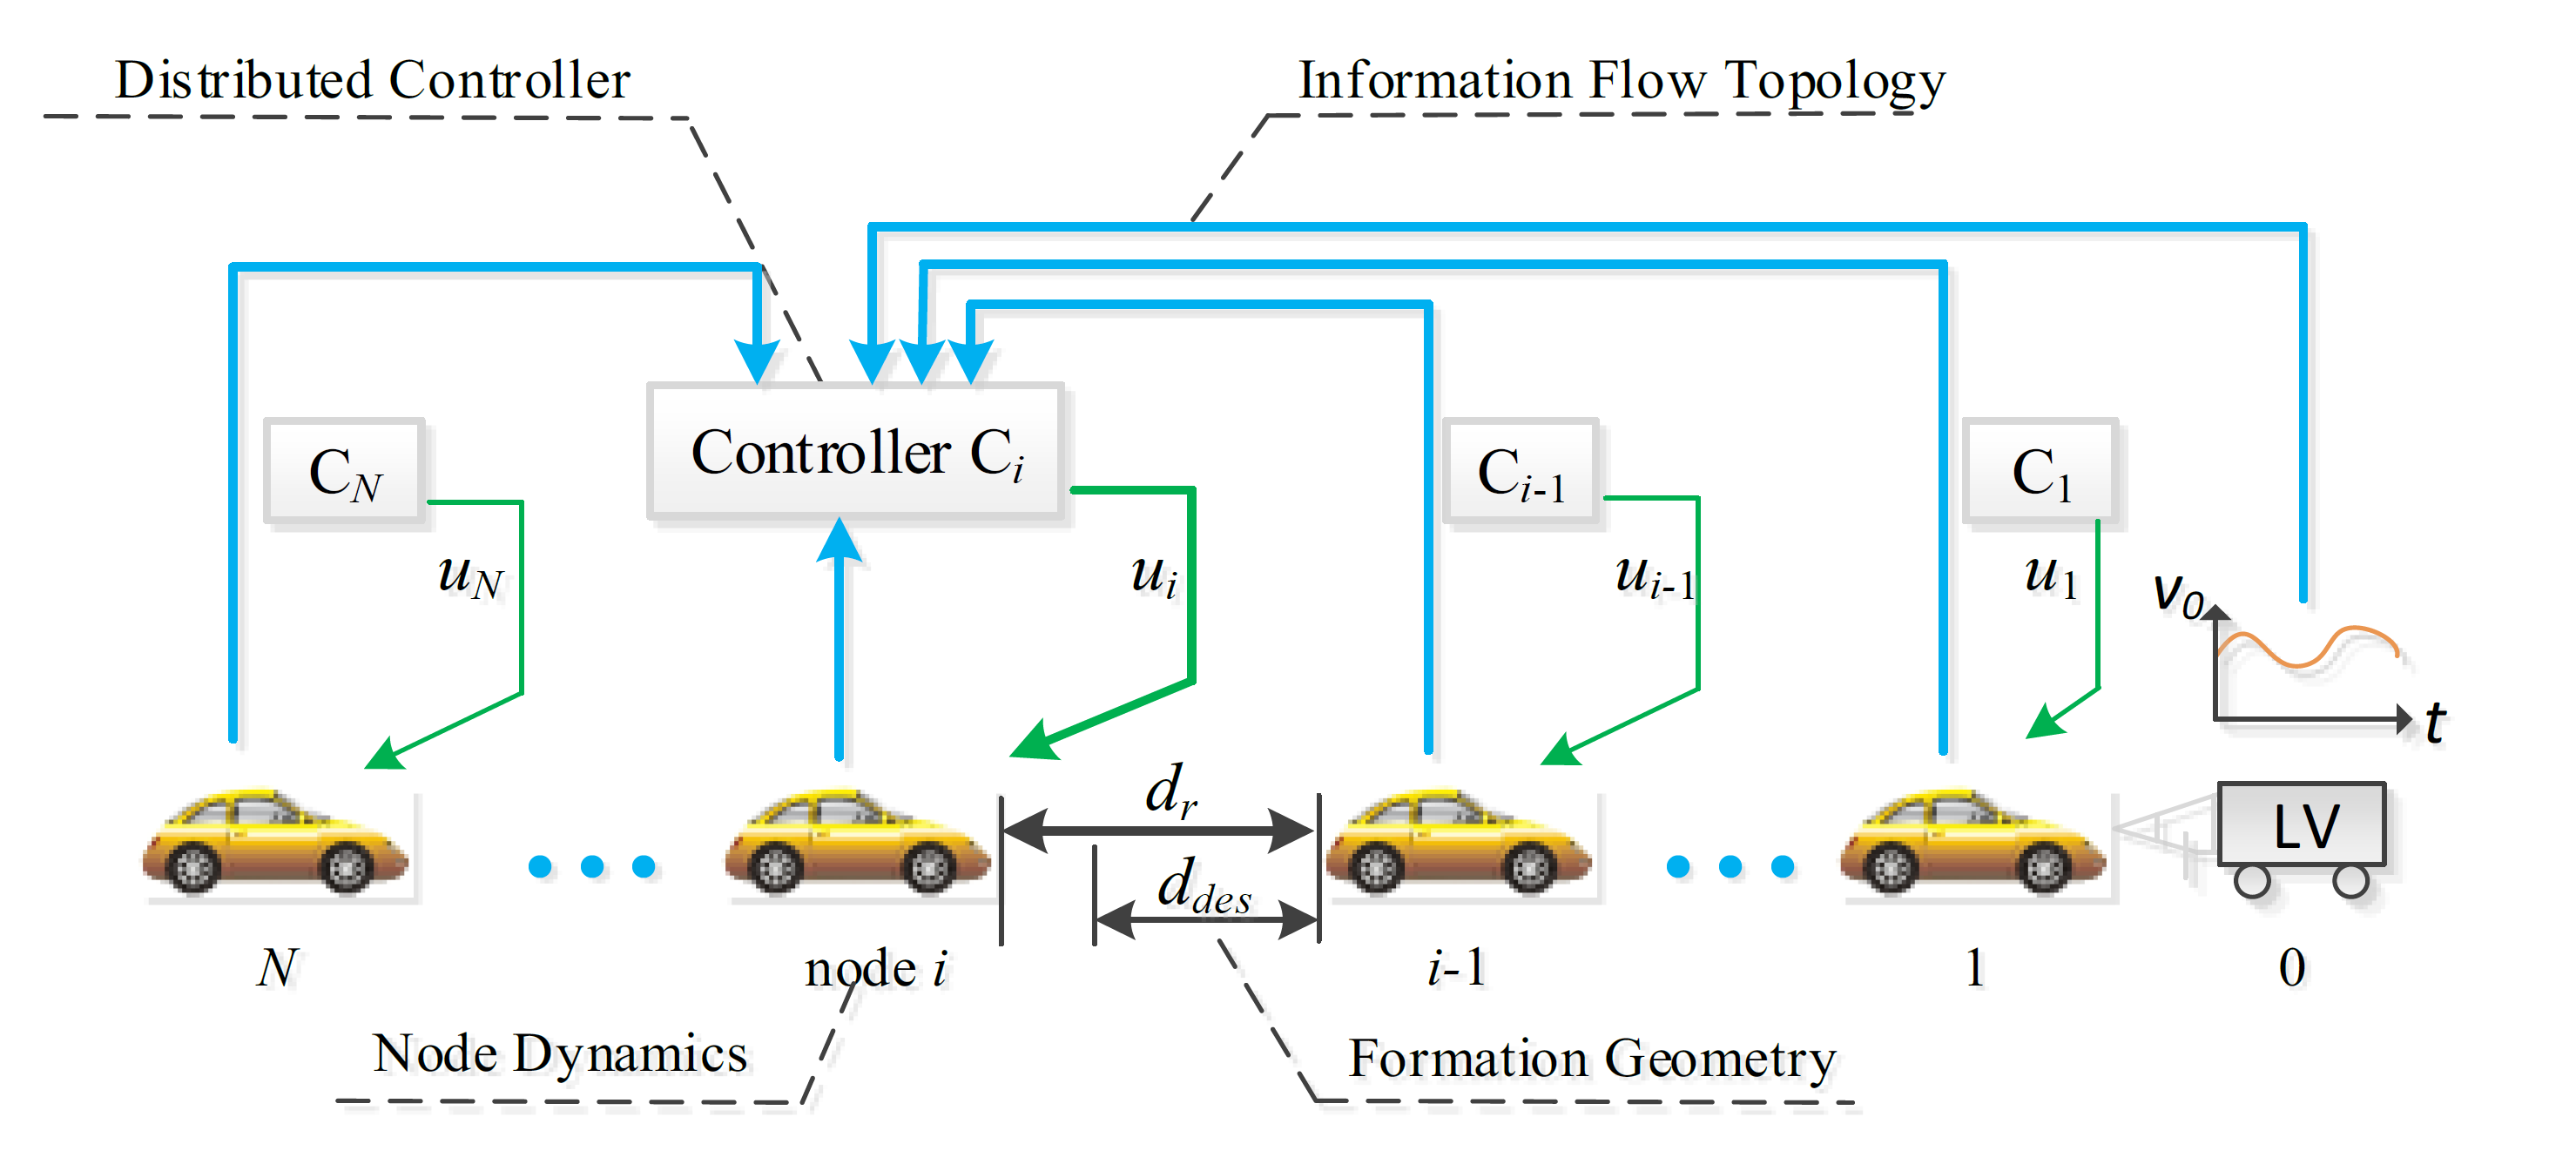
\includegraphics[scale=0.2]{Images/intro-platoon.png}
	\caption{شمای کلی از نحوه کار سیستم‌های دسته‌ای}\label{Fig intro platoon}
\end{figure}

همانطور که در شکل \ref{Fig intro platoon} مشاهده می‌شود هر ماشین باید به اندازه کافی هوشمند باشد تا بتواند موقعیت خود را بدست آورده و باید حداقل به یک یا تعداد بیشتر خودروها ارسال کند و سپس با توجه به موقعیت ارسالی از هر ماشین به کمک یک کنترلر که در هر ماشین قرار دارد به موقعیت مطلوب برسد تا آن‌ها بتوانند با هم در مسیر مطلوب حرکت کنند.

در این مقوله برای استفاده بهینه از این خودروهای خودران در بزرگراه‌ها به کنترل دسته‌ای آن‌ها روی می‌آورند. مانند شکل \ref{Fig intro platoon} به طوری که در این دسته یک رهبر\LTRfootnote{leader} و بقیه ماشین‌ها دنبال‌کننده‌ی\LTRfootnote{follower} رهبر هستند.

علاوه بر این موضوع، برنامه‌ریزی برای رسیدن به بهترین مسیر نیز یکی دیگر از نکات مهم برای حمل و نقل و خودروهای هوشمند است. منظور از برنامه‌ریزی، یافتن یک برنامه معقول برای اجرای آن است. برای مسیریابی روش‌های مختلفی همانند میدان پتانسیل\LTRfootnote{potential field}، روش نمونه‌گیری\LTRfootnote{sampling based method}، کنترل پیشبین\LTRfootnote{model predictive control}، روش‌های احتمالاتی\cite{lefkopoulos2019using} و یادگیری\LTRfootnote{learning} وجود دارند که هر کدام به طور کامل در فصل \ref{ch path planning} به طور کامل توضیح داده شده‌اند.

\section{طرح مسئله}
برای پیاده‌سازی مسئله طرح شده با هدف کنترل اجماع و مسیریابی ربات‌ها، همانطور که گفته شد از برنامه \verb|MATLAB| و \verb|toolbox simulation robotics mobile| استفاده شده است. برای تست‌های اولیه نتایج کنترل تک ربات و در انتها با 3 و 4 ربات پلتون و مسیریابی آن انجام شده است. مدل ربات‌ها به صورت دیفرانسیلی\LTRfootnote{differential} در نظر گرفته شده است که به معادلات آن در فصل \ref{ch one robot} پرداخته شده است.

اطلاعات ما از محیط از سوی دیگاه پرنده\LTRfootnote{bird's eye view} از محیط گرفته می‌شود. مسیریابی‌ها قابل برنامه‌ریزی به صورت آفلاین، با اجرای فایل \verb|.m| هر الگوریتم و سپس اجرا شبیه‌سازی مربوطه و همینطور به صورت آنلاین قابل برنامه‌ریزی است. سعی شده است که انواع روش‌های مسیریابی پیاده‌سازی و مورد بررسی قرار گیرند. همچنین تا سطح موانع متحرک، مسیریابی و کنترل اجماع به صورت بلادرنگ\LTRfootnote{real time} ارتقا یافته است.
روش‌های مسیریابی استفاده شده به شرح زیر هستند:
\begin{enumerate}
	\item میدان پتانسیل
	\item روش‌های نمونه‌برداری و ابتکاری
	\begin{itemize}
		\item \verb|BFS|\LTRfootnote{Breadth first search}
		\item \verb|search first best Greedy|
		\item $A^*$
	\end{itemize}
	\item روش‌های یادگیری تقویتی\LTRfootnote{Reinforcement learning}
	\begin{itemize}
		\item \verb|learning Q|
	\end{itemize}
\end{enumerate}

پیاده‌سازی این روش‌ها دارای مهارت و دانش در مورد هوش مصنوعی و روش تبدیل کردن مسئله مسیریابی برای ربات‌ها به یک مسئله دارای حالت\LTRfootnote{state}، اقدامات\LTRfootnote{actions} و تبادل اطلاعات بین ربات‌ و محیط است که در فصل \ref{ch path planning} به طور مفصل در مورد آن‌ها صحبت شده است.

نکته قابل توجه، ساده‌نویسی کد است به طوری که به راحتی بتوان آن را با زبان \verb|C| نیز درک و نوشت تا بتواند بر روی دو ربات مستقر در آزمایشگاه بلادرنگ که مدل آن‌ها نیز دیفرانسیلی است، پیاده‌سازی کرد.

\section{قالب‌بندی پایان‌نامه}






















